\documentclass[12pt,a4paper]{article}
\usepackage[slovene]{babel}
\usepackage{amsfonts,graphicx}
% Mno"zice realnih, naravnih in kompleksnih "stevil
\def\RR{\mathbb{R}}
\def\NN{\mathbb{N}}
\def\CC{\mathbb{C}}
\addtolength{\textheight}{4cm}
\addtolength{\voffset}{-2cm}

\newtheorem{definicija}{Definicija}
\newtheorem{primer}{Primer}
% Odebeljene "crke v math na"cinu 
% (povezto po L.L. Schumaker - makro
% za St. Malo Proceedings
\def\bfm#1{{\dimen0=.01em\dimen1=.009em\makebold{$#1$}}}

\def\makebold#1{\mathord{\setbox0=\hbox{#1}%
       \copy0\kern-\wd0%
       \raise\dimen1\copy0\kern-\wd0%
       {\advance\dimen1 by \dimen1\raise\dimen1\copy0}\kern-\wd0%
       \kern\dimen0\raise\dimen1\copy0\kern-\wd0%
       {\advance\dimen1 by \dimen1\raise\dimen1\copy0}\kern-\wd0%
       \kern\dimen0\raise\dimen1\copy0\kern-\wd0%
       {\advance\dimen1 by \dimen1\raise\dimen1\copy0}\kern-\wd0%
       \kern\dimen0\raise\dimen1\copy0\kern-\wd0%
       \kern\dimen0\box0}}
\pagestyle{empty}

\begin{document}

\begin{center}
  IZPIT IZ NUMERI"CNE MATEMATIKE\\
  19. september 2003
\end{center}
\vspace{2cm}

\begin{enumerate}
  \item S "colna so izmerili globino jezera v petih to"ckah (glej sliko)
  $$\begin{array}{l|rrrrr}
      x & 0 & 10 & 20 & 30 &40\\ \hline
      y & 0 & -15 & -18 & -17 & 0
     \end{array}
  $$
  \begin{figure}[h]
  \begin{center}
       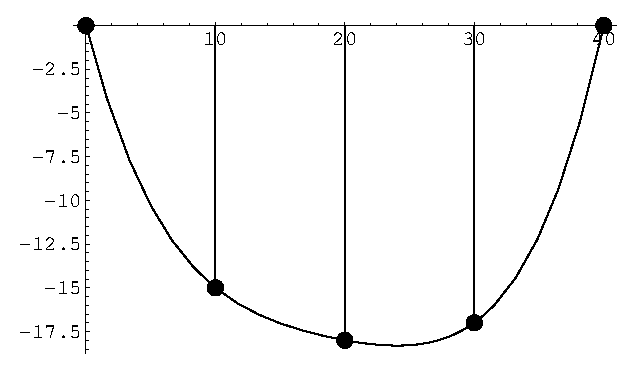
\includegraphics[width=7cm]{jezero.eps} 
  \end{center}
  \end{figure}
  \begin{itemize}
    \item[a)] Dolo"cite interpolacijski polinom skozi izmerjene to"cke,
    ki predstavlja pribli"zno obliko preseka skozi jezero. 

    \item[b)] Na podlagi izmerjenih podatkov s sestavljenim trapeznim
    pravilom izra"cunajte plo"s"cino preseka jezera.
 
     \item[c)] Ocenite globino jezera tako, da poi"s"cete minimum
     interpolacijskega polinoma iz to"cke a). Metodo za izra"cun
     minimuma izberite sami. 

  \end{itemize}
  
  \item Re"sujete za"cetni problem 
  \begin{eqnarray*}
    y' &=& z,\quad y(0)=1,\\
    z' &=& -y, \quad z(0)=0.
  \end{eqnarray*}
 
   \begin{itemize}
    \item[a)] Poi"s"cite to"cno re"sitev problema. (Namig: Sistem
    prevedite na eno samo diferencialno ena"cbo drugega reda.) 

    \item[b)] Na intervalu $[0,1]$ poi"s"cite pribli"zno re"sitev z 
    Eulerjevo metodo
    s korakom $h=0.25$.

    \item[c)] Kolik"sna je druga norma globalne napake re"sitve iz to"cke b)
    v to"cki $x=1$. 

  \end{itemize}
\end{enumerate}
Ustni izpit bo v torek 30. 9. v pisarni Bojana Orla. To"cna ura bo objavljena 
kasneje.
\end{document}
